\chapter{Umsetzung von Kommunikationsschemen über Kafka} 
\label{chap:Kafka}
\newcommand{\C}{\textit{Consumer}}
\newcommand{\Cn}{\textit{Consumern}}
\newcommand{\CG}{\textit{Consumer Group}}
\newcommand{\CGs}{\textit{Consumer Groups}}
\newcommand{\T}{\textit{Topic}}
\newcommand{\Tcs}{\textit{Topics}}
\newcommand{\Pt}{\textit{Partition}}
\newcommand{\Pts}{\textit{Partitionen}}
\newcommand{\Pd}{\textit{Producer}}
\newcommand{\Evs}{\textit{Events}}
\newcommand{\Ev}{\textit{Event}}
Um unsere Applikation skalierbar aufsetzen zu können, musste auf die Skalierbarkeit der Kommunikation zwischen den Microservices geachtet werden. In diesem Kapitel wird beschrieben, wie eine skalierbare Kommunikation über Kafka umgesetzt wurde. Hierfür werden zunächst die benötigten Grundlagen bezüglich Kafka beschrieben und anschließend wird auf die Realisierung von zwei Kommunikationsschemen mithilfe von Kafka eingegangen.
\section{Grundlagen Kafka}
Die in diesem Abschnitt beschriebenen Grundlagen stammen aus \cite{KafkaIntro} und \cite{KafkaDoku}.
\subsection{Registrieren eines Consumers}
Wird eine Nachricht über eine Kafka-Instanz verbreitet, so ist sie einem \T\ zugeordnet.
Möchte eine Komponente von Kafka Nachrichten erhalten, muss sie sich als \C\ registrieren. Hierbei muss sie mindestens ein \T\ angeben, an dem sie interessiert ist, sowie eine \CG. Wird nun eine Nachricht über Kafka verbreitet, wird ein \C\ jeder \CG, der an dem \T\ der Nachricht interessiert ist, ausgewählt und die Nachricht an diesen \C\ weitergeleitet. Abbildung \ref{fig:exampleKafkaConsumerRegistration} zeigt ein Beispiel für die Zuordnung von \Cn\ zu \CGs\ und die Registrierung der \C\ bei verschiedenen \Tcs. Wird in diesem Beispiel ein Nachricht für \T\ 2 hinterlegt, so werden \C\ 1 oder \C\ 2, sowie \C\ 4 informiert. Wird allerdings eine Nachricht für \T\ 1 hinterlegt, wird nur \C\ 1 oder \C\ 2 informiert.
\begin{figure}
	\caption{Beispiel für die Zuordnung von \Cn\ zu \CGs\ und \Tcs.}
	\label{fig:exampleKafkaConsumerRegistration}
	\centering
	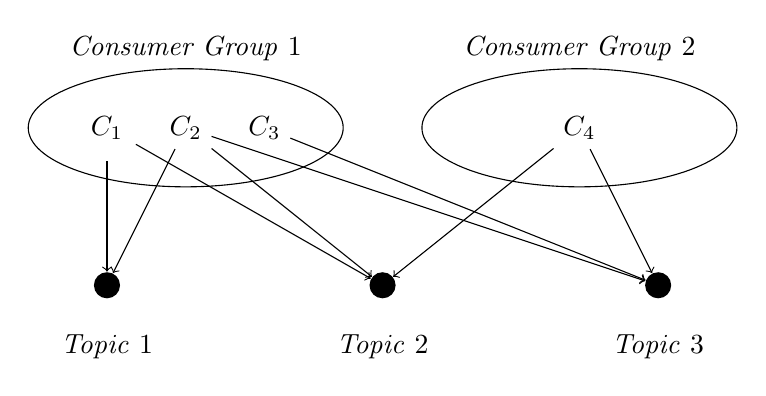
\begin{tikzpicture}
		\draw (0,0) ellipse (2cm and 0.75cm);
		\node (CG2) at (0,1) {\CG\ 1};
		\draw (5,0) ellipse (2cm and 0.75cm);
		\node (CG2) at (5,1) {\CG\ 2};
		\node[fill=black, circle] (T1) at (-1,-2) {};
		\node[fill=black, circle] (T2) at (2.5,-2) {};
		\node[fill=black, circle] (T3) at (6,-2) {};
		\node[below=0.5cm] at (T1) {\T\ 1};
		\node[below=0.5cm] at (T2) {\T\ 2};
		\node[below=0.5cm] at (T3) {\T\ 3};
		\node[circle, minimum size=0.1cm] (C1) at (-1,0) {$C_1$};
		\node (C2) at (0,0) {$C_2$};
		\node (C3) at (1,0) {$C_3$};
		\node (C4) at (5,0) {$C_4$};
		\path[->] (C1) edge (T1) edge (T2)
		(C2) edge (T1) edge (T2) edge (T3)
		(C3) edge (T3)
		(C4) edge (T2) edge (T3);
	\end{tikzpicture}
\end{figure}
\subsection{Nachrichtenverteilung}
Ein \T\ von Kafka ist in mehrere \Pts\ unterteilt. Die Anzahl der \Pts\ muss angegeben werden, wenn ein \T\ erstellt wird. \\
Haben sich mehrere \C\ einer \CG\ bei Kafka registriert, um Nachrichten für ein \T\ zu erhalten, so werden die \Pts\ zunächst auf die \C\ der \CG\ verteilt. Erhält Kafka nun eine Nachricht für das \T, kann entweder vom \Pd\ - also dem Sender der Nachricht - festgelegt werden, in welche Partition die Nachricht gelegt werden soll, oder Kafka teilt die Nachricht so einer Partition zu, dass die Nachrichten möglichst gleichmäßig auf die \Pts\ verteilt sind. Nachdem die Nachricht einer \Pt\ zugeordnet ist, wird sie dem \C\ einer jeden \CG\ übermittelt, dem die \Pt\ zugeteilt ist. \\
Für die Zuordnung der \Pts\ zu den \Cn\ einer jeden \CG\ wird eine Zuordnungsstrategie verwendet. Hier liefert Kafka die beiden Strategien \glqq range\grqq\ und \glqq roundrobin\grqq\ mit, von denen eine ausgewählt werden kann. Alternativ lässt sich eine eigene Zuordnungsstrategie definieren.
\section{Realisierung der Kommunikationsschemen}
In unserem Projekt \glqq Hamaube\grqq\ haben wir die Semantik der Nachrichten so gewählt, dass sie als \Evs\ zu verstehen sind. Diese \Evs\ können potentiell von einer beliebigen Instanz ausgelesen werden. So ist beispielsweise unsere Analyseinstanz an mehrere \Tcs\ angeschlossen, um Analysen über die Nutzung von Hamaube bzw. die Twitterdaten durchzuführen. \\
\\
Trotz dieser \Ev-Charakteristik haben viele Nachrichten ein primäres Ziel. So hat beispielsweise ein \Ev, das signalisiert, dass ein Anwender eine Webserver-Instanz nach seiner Timeline gefragt hat, das primäre Ziel, dass es von einer beliebigen Cassandra\_Reader-Instanz aufgenommen wird, um die Einträge der Timeline aus der Datenbank zu laden. Anschließend sollte diese Cassandra\_Reader-Instanz ein \Ev\ verschicken, das signalisiert, welche Einträge dem Anwender angezeigt werden sollen. Dieses \Ev\ hat wiederum das primäre Ziel, dass die entsprechende Webserver-Instanz die Anfrage des Nutzers beantworten kann. Im Folgenden wird die Komponente, die das \Ev\ primär erhalten soll, Kommunikationspartner genannt.
\subsection{Beliebiger Kommunikationspartner}
Für viele Nachrichten, die Hamaube über Kafka verschickt, reicht es, wenn eine beliebige Instanz einer bestimmten Gruppe von Servern das Event erhält. Wenn beispielsweise eine Webserver-Instanz eine Cassandra\_Reader-Instanz darüber informieren möchte, dass die Einträge einer Timeline geladen werden sollen, ist für die Webserver-Instanz egal, welche Cassandra\_Reader-Instanz das Event zur Bearbeitung der Anfrage erhält.\\
Soll ein beliebiger Kommunikationspartner für ein Event ausgewählt werden, kann das Event von Kafka einer beliebigen Partition zugeteilt werden und eine der beiden Standard Zuordnungsstrategien gewählt werden, um die Partitionen den \Cn\ der \CG\ zuzuordnen.
\subsection{Ausgewählter Kommunikationspartner}
In einigen Fällen ist das \Ev\ allerdings primär nur für eine Instanz entscheidend. So sollte das \Ev, dass die Einträge einer Timeline enthält beispielsweise möglichst direkt die Webserver-Instanz erreichen, an der die Timeline angefragt wurde. Um dies zu realisieren, könnte die Webserver-Instanz der Anfrage ihre ID hinzufügen und dann das Antwort-\T\ nach ihrer ID filtern. Diese Lösung würde allerdings dazu führen, dass die Kommunikation nicht mehr skalierbar wäre, da dann jede Webserver-Instanz jede Antwort auf jede Anfrage erhalten müsste und zum Filtern der Antworten bearbeiten müsste. Dies ließe sich nicht skalierbar realisieren. Die \C\ müssen also der selben \CG\ zugeordnet sein. \\
Um nun zu gewährleisten, dass die Webserver-Instanz, die die Anfrage gestellt hat, die Antwort erhält, muss die Antwort zum einen in eine feste \Pt\ gelegt werden und zum anderen musste eine Strategie für die Zuordnung von Partitionen auf die \C\ implementiert werden, mit der garantiert werden kann, dass die Antwort auch bei erneuter Verteilung der \Pts\ beim richtigen \C\ landet. Dies können beide von Kafka mitgelieferten Verteilungsstrategien nicht gewährleisten, wie in Abbildung \ref{fig:roundrobin} beispielhaft für das \glqq roundrobin\grqq-Verfahren dargestellt ist.
\begin{figure}
	\caption{Beispiel für die Umverteilung der Partitionen mit dem \glqq roundrobin\grqq\ Verfahren: Zwischen Zustand 1 und Zustand 2 wurde der Consumer 2 entfernt.}
	\label{fig:roundrobin}	
	\centering
	\textbf{Zustand 1:} \\
	\begin{tabular}{c | c | c}
		Consumer 1 & Consumer 2 & Consumer 3 \\
		\hline
		Partition 1 & Partition 2 & Partition 3 \\
		Partition 4 & Partition 5
	\end{tabular} \\[0.5cm]
	\textbf{Zustand 2:} \\
	\begin{tabular}{c | c}
	Consumer 1 & Consumer 3 \\
	\hline
	Partition 1 & Partition 2 \\
	Partition 3 & Partition 4 \\
	Partition 5
	\end{tabular}
\end{figure} \\
\\
Wird eine Webserver-Instanz von Hamaube gestartet, muss ihr eine Partitionsnummer als Argument übergeben werden. Registriert sich die Webserver-Instanz bei Kafka als Consumer, kann sie eine ID übergeben, die später an den Verteilungsalgorithmus für die Partitionen weitergegeben wird. Durch die ID kann der selbst implementierte Verteilungsalgorithmus erkennen, welche Partition diesem Consumer zugeordnet werden muss. Ist eine Partition vorhanden, für die kein Consumer existiert, dessen ID die Nummer der Partition enthält, wird die Partition einem beliebigen Consumer zugeordnet.\\
\\
Schickt eine Webserver-Instanz nun eine Anfrage an eine Cassandra\_Reader-Instanz, enthält diese Anfrage ein Feld, das die Partition angibt, in die die Antwort gelegt werden soll. Durch den Verteilungsalgorithmus für die Partitionen ist garantiert, dass der Webserver-Instanz, solange sie erreichbar ist, diese Partition zugeordnet ist, sodass nur sie die Antwort erhält. Ist die Webserver-Instanz nicht mehr erreichbar, wird ihre Partition einer anderen Webserver-Instanz zugeordnet, die die Antwort erhält und verwirft, da sie die Anfrage nicht gestellt hat. Die Antwort geht in diesem Falle also verloren.

\section{Microservice übergreifendes Datenformat}
Wir haben beschlossen, Daten von Twitter in unserer Applikation zu verarbeiten. Hierfür haben wir einen Twitterstream angeschlossen, der Tweets aus Twitter in eines unserer Topics legt. Unter anderem sollte der Cassandra-Reader sich auf diesem Topic subscriben und die Tweets in Cassandra speichern.\\
Da zu Beginn des Projektes nicht klar war, was für Analysen wir später auf den Daten durchführen könnten und welche Teile der Twitterdaten wir dafür benötigen könnten, haben wir beschlossen, alle Daten über die Tweets von Twitter zu speichern und das Datenformat von Twitter für unsere Kommunikation und die Datenhaltung in Cassandra zu übernehmen. \\
\\
Wir mussten feststellen, dass das Format der Tweet-Daten von Twitter eine sehr große, verschachtelte Struktur ist, in der häufig $null$-Werte auftauchen. Die $null$-Werte haben dafür gesorgt, dass sich die Definition des Datenformats manuell nur schwer aus den Daten extrahieren ließ. Twitter stellt eine Api für die Schnittstelle zur Verfügung, aber auch hier wäre es sehr aufwändig gewesen, das gesamte Datenformat zu entnehmen.\\
\\
Um dennoch eine Definition des Datenformats zu finden, haben wir einen Parser geschrieben, der als Eingabe eine Datei mit Tweets von Twitter entgegen nimmt und aus diesen Daten das Datenformat in Form von Cql-Typ-Definitionen ausgibt. Das Ergebnis enthält alle Felder mit Typ-Angabe, für die in den Tweet-Daten aus der Datei mindestens ein Eintrag mit einem Wert außer $null$ gefunden wurde. Nur ein paar Felder konnten nicht übernommen werden, da sie immer mit $null$ befüllt waren. Für diese Felder ließ sich in der Twitter-Api nachlesen, dass diese $deprecated$ sind - also nicht mehr genutzt werden. Die Felder, die wir nicht in unsere Datenstruktur übernommen haben, können also keine relevanten Information enthalten.